\documentclass[10pt]{article}
\usepackage[margin=.75in]{geometry}\usepackage{amsmath,tikz,hyperref}
\setlength{\parindent}{0pt}\setlength{\parskip}{7pt}
\begin{document}
\textbf{Cached-inverse coefficient traversal}\hfill2026-10-31\\T-1167. Producer proof; independent source-fidelity review pending.

The full coefficient traversal composes the preceding word update through a size-indexed array. The inverse is computed once before traversal and passed unchanged through every step.

For any valid event sequence $E$, the checked invariant is
\[
 \operatorname{decode}(\mathrm{out}'_i)=\operatorname{decode}(\mathrm{out}_i)
 +\sum_{(k,j)\in E}\mathbf{1}_{i=j}\,c_k\binom{k}{j}a^jb^{k-j}s^{-1}.
\]
Every intermediate array remains canonical. The transform theorem starts with a zero array and supplies the generated inverse. Assumptions: $0\le n\le6$, prime $1<p<2^{31}$, canonical coefficients and parameters, and nonzero scale.
\begin{center}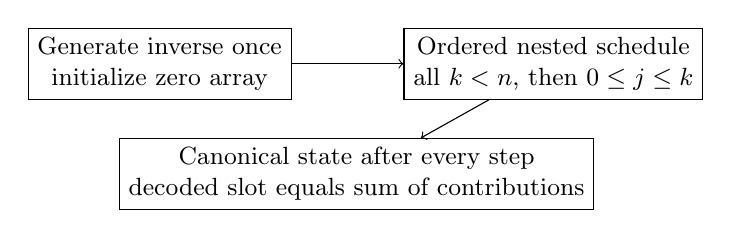
\begin{tikzpicture}[every node/.style={draw,align=center,font=\small}]
\node(a)at(0,0){Generate inverse once\\initialize zero array};
\node(b)at(5,0){Ordered nested schedule\\all $k<n$, then $0\le j\le k$};
\node(c)at(2.5,-1.4){Canonical state after every step\\decoded slot equals sum of contributions};
\draw[->](a)--(b);\draw[->](b)--(c);
\end{tikzpicture}\end{center}
For every supported length $0,\ldots,6$, a separate theorem identifies the schedule with the source's nested ranges in their exact order. It has no repeated index pairs and has $n(n+1)/2$ events. The six-coefficient case has 21 updates (derived schedule count, not measured time).

Seven main declarations and eleven fixed controls passed; all 18 named axiom readbacks contain only standard Lean axioms. The four native module checks passed on their first attempts. Controls include empty, constant, quadratic, scaled quadratic, zero, identity and shifted quintic inputs. Modulo 17,
\[
 [1,2,3,4,5,6]\quad\xrightarrow{x\mapsto x+1}\quad[4,2,3,16,1,6].
\]
Omitting the highest input row changes that output. These are formal controls, not cohort measurements.

Source: \texttt{projective\_law\_gate.rs} transform and the preceding storage, arithmetic, inverse and symbolic-loop proofs. Primary references: \href{https://lean-lang.org/doc/api/Init/Data/List/Control.html}{Lean list traversal} and \href{https://lean-lang.org/doc/api/Init/Data/Array/Set.html}{Array.set semantics}.

The expression above sums over the exact nested schedule. Identifying it with the existing polynomial-composition theorem, then binding trailing-zero trimming and fixed-size divisor copying, are the next steps. This is a logical source model, not compiled-Rust equivalence. Existing compiled dependencies remain in the trust boundary.

Native exits and unchanged source/dependency hashes accompany the PDF, editable diagram, status JSON and custody. No scientific campaign, timing or cost ratio; cohort and authorization limits unchanged.
\end{document}
